%\documentclass{article}
%\usepackage{subfig}
%\usepackage{tikz}
%\usepackage{siunitx}
%\begin{document}
%\newcommand{\imsize}{\linewidth}
%\newlength\imagewidth % needed for scalebars
%\newlength\imagescale % needed for scalebars
%\begin{figure}
%	\centering
%%%%%%%%%%%%%%%%%%%%%%%%%%%%%
	\renewcommand{\imsize}{.33\linewidth}
	\pgfmathsetlength{\imagewidth}{\imsize} % desired display width of image
	\pgfmathsetlength{\imagescale}{\imagewidth/1024} % pixel width of image
	\centering
		\subfloat[Three uncorrected and independent projection images from subscans s$_1$--s$_3$, each with a size of 1024\(\times\)1024 pixels at a resolution of \SI{1.48}{\micro\meter\per pixel}, each covering a FOV of \SI{1.52}{\milli\meter}. Subscans s$_1$ and s$_2$ overlap each other by 141 pixels (red and green overlay), subscans s$_2$ and s$_3$ overlap each other by 138 pixels (blue and yellow overlay). 5244 projections  over a rotation of \SI{180}{\degree} have been acquired for all subscans.]{%
			\label{fig:s1}%
			% --------------------------------------------------------------
			% Cutline between SubScan 1 and 2: 141 pixels
			% Cutline between SubScan 2 and 3: 138 pixels
			% --------------------------------------------------------------
			\begin{tikzpicture}[x=\imagescale,y=-\imagescale]%
				\node[anchor=north west,inner sep=0pt,outer sep=0pt] at (0,0)%
					{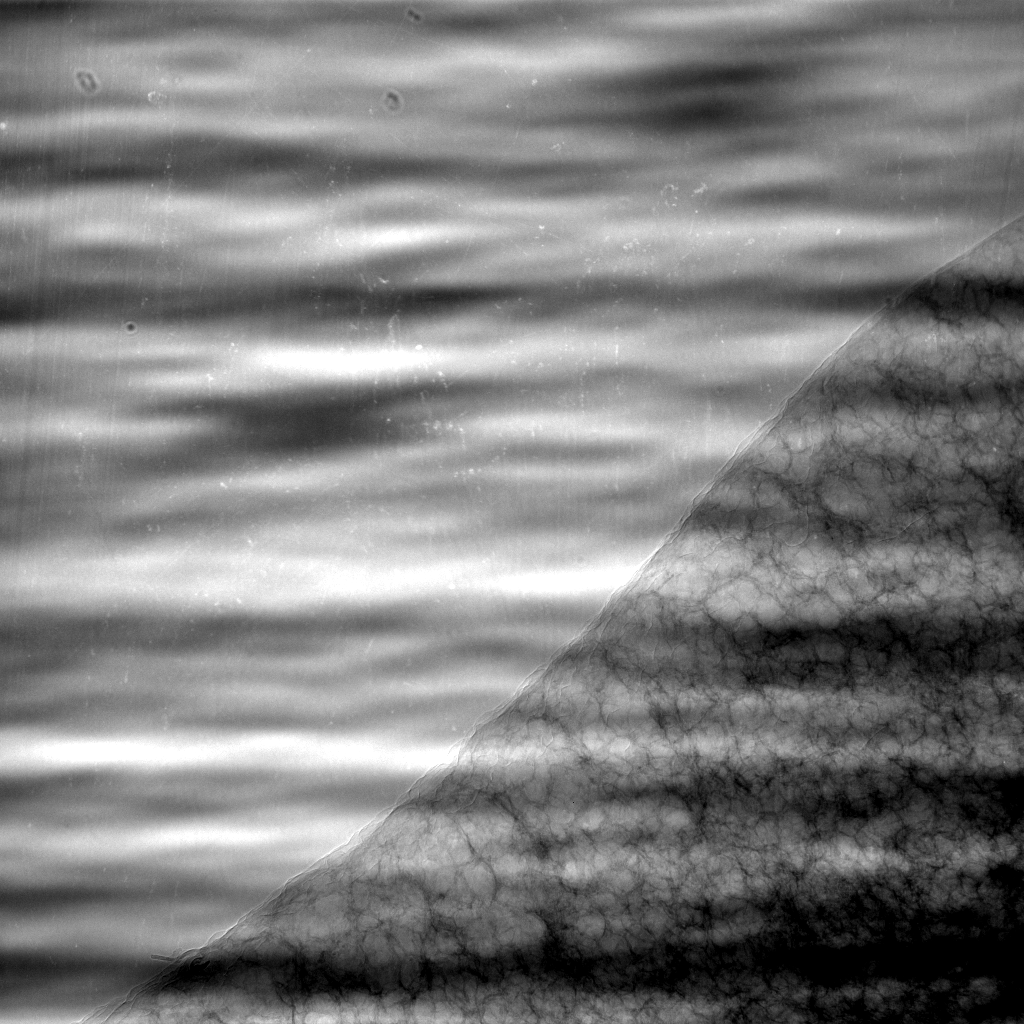
\includegraphics[width=\imagewidth]{R108C21Cb_s13358_normalize}};%
				\def\overlap{141}%
				\fill [red, nearly transparent] (1024-\overlap,1) rectangle (1024,1024);%
				\draw (1024-\overlap,1) rectangle (1024,1024);%
			\end{tikzpicture}%
			\begin{tikzpicture}[x=\imagescale,y=-\imagescale]%
				\node[anchor=north west,inner sep=0pt,outer sep=0pt] at (0,0)%
					{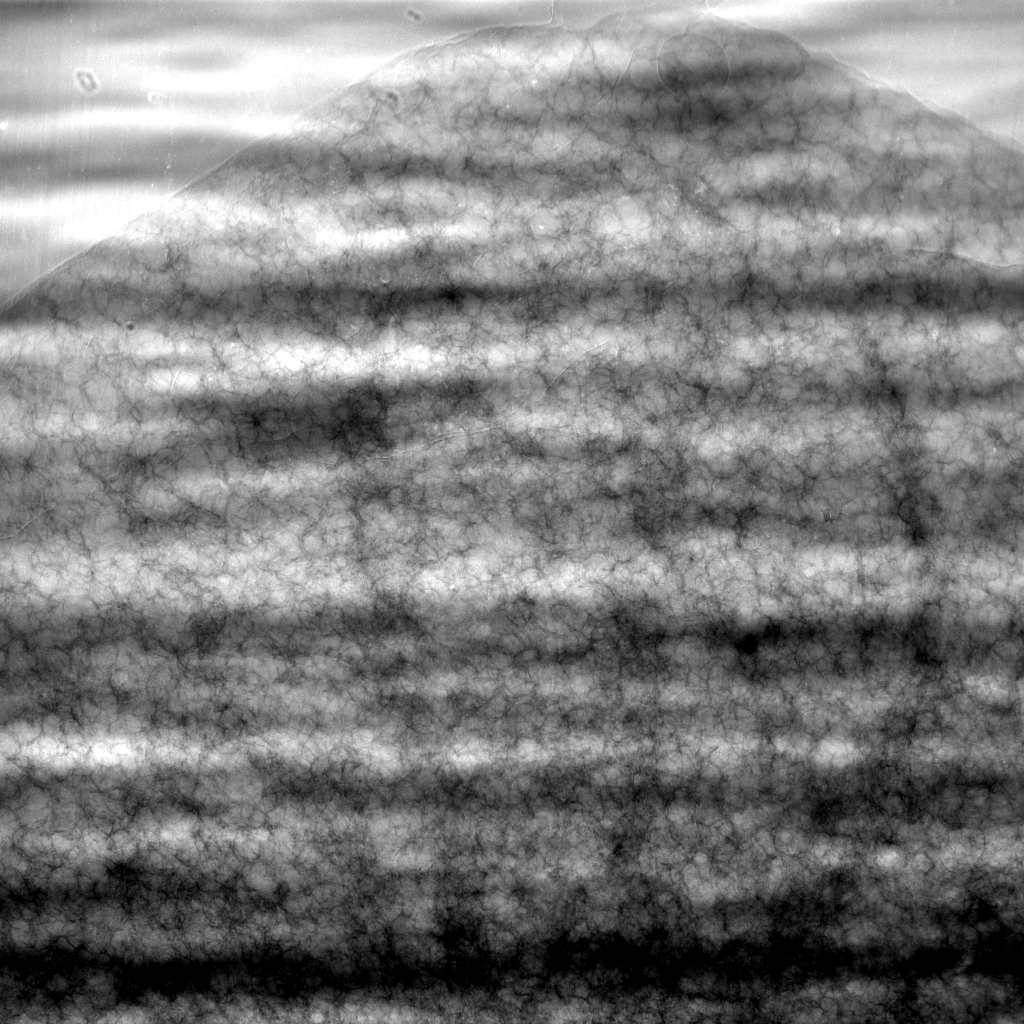
\includegraphics[width=\imagewidth]{R108C21Cb_s23358_normalize}};%
				\def\overlap{141}%
				\fill [green, nearly transparent] (1,1) rectangle (\overlap,1024);%
				\draw (1,1) rectangle (\overlap,1024);%
				\def\overlap{138}%
				\fill [blue, nearly transparent] (1024-\overlap,1) rectangle (1024,1024);%
				\draw (1024-\overlap,1) rectangle (1024,1024);%
			\end{tikzpicture}%
			\begin{tikzpicture}[x=\imagescale,y=-\imagescale]%
				% place image (integer coordinates refer to pixel centers):
				\node[anchor=north west,inner sep=0pt,outer sep=0pt] at (0,0)%
					{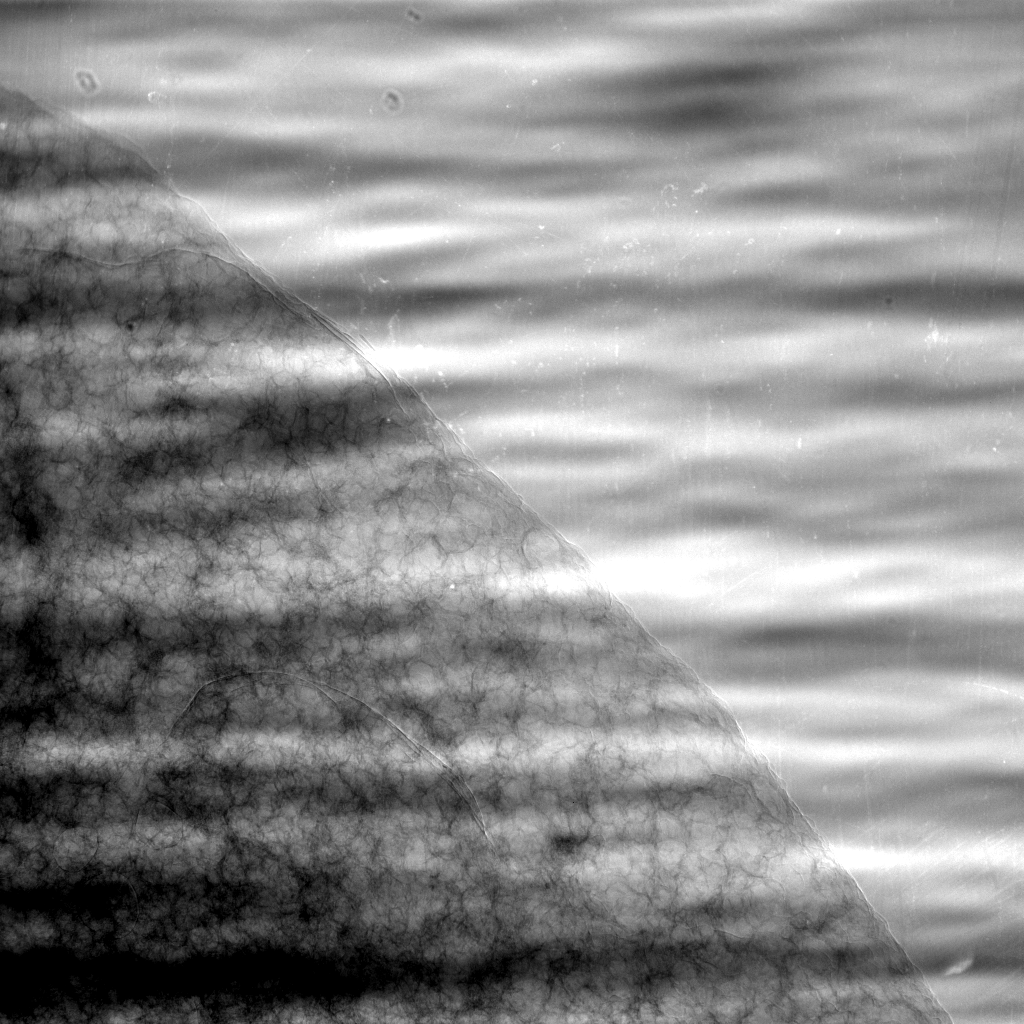
\includegraphics[width=\imagewidth]{R108C21Cb_s33358_normalize}};%
				\def\overlap{138}%
				\fill [yellow, nearly transparent] (1,1) rectangle (\overlap,1024);%
				\draw (1,1) rectangle (\overlap,1024);%
				\draw[|-|,color=white] (1,200) -- (1024,200) node [midway,above] {\SI{1.51552}{\milli\meter}};%
				\def\x{924}% 1024 - 100
				\def\y{922}% 1024 * .9 = 921.6
				\def\bar{338}% 100 px = 148 um
				\draw[|-|,color=white] (\x-\bar,\y) -- (\x,\y) node [midway,above] {\SI{500}{\micro\meter}};%
			\end{tikzpicture}%
			\label{fig:subscans}%
			}\\%
		\renewcommand{\imsize}{\linewidth}%
		\pgfmathsetlength{\imagewidth}{\imsize} % desired displayed width of image
		\pgfmathsetlength{\imagescale}{\imagewidth/2793}% pixel width of image
		\subfloat[Merged and corrected image from the three subscans shown in subfigure~\subref{fig:subscans}. Each merged projection has a size of 2793\(\times\)1024 pixels at a resolution of \SI{1.48}{\micro\meter\per pixel}. The width of the merged projections is slightly smaller than three times the width of the subscans due to the overlap needed to merge the projections (2793~px$=3\cdot3072$~px$-141$~px$-138$~px). Since the x-ray beam is extremely stable, the bands visible in the raw projections can be eliminated.]{%
			\begin{tikzpicture}[x=\imagescale,y=-\imagescale]%
				\node[anchor=north west,inner sep=0pt,outer sep=0pt] at (0,0)%
					{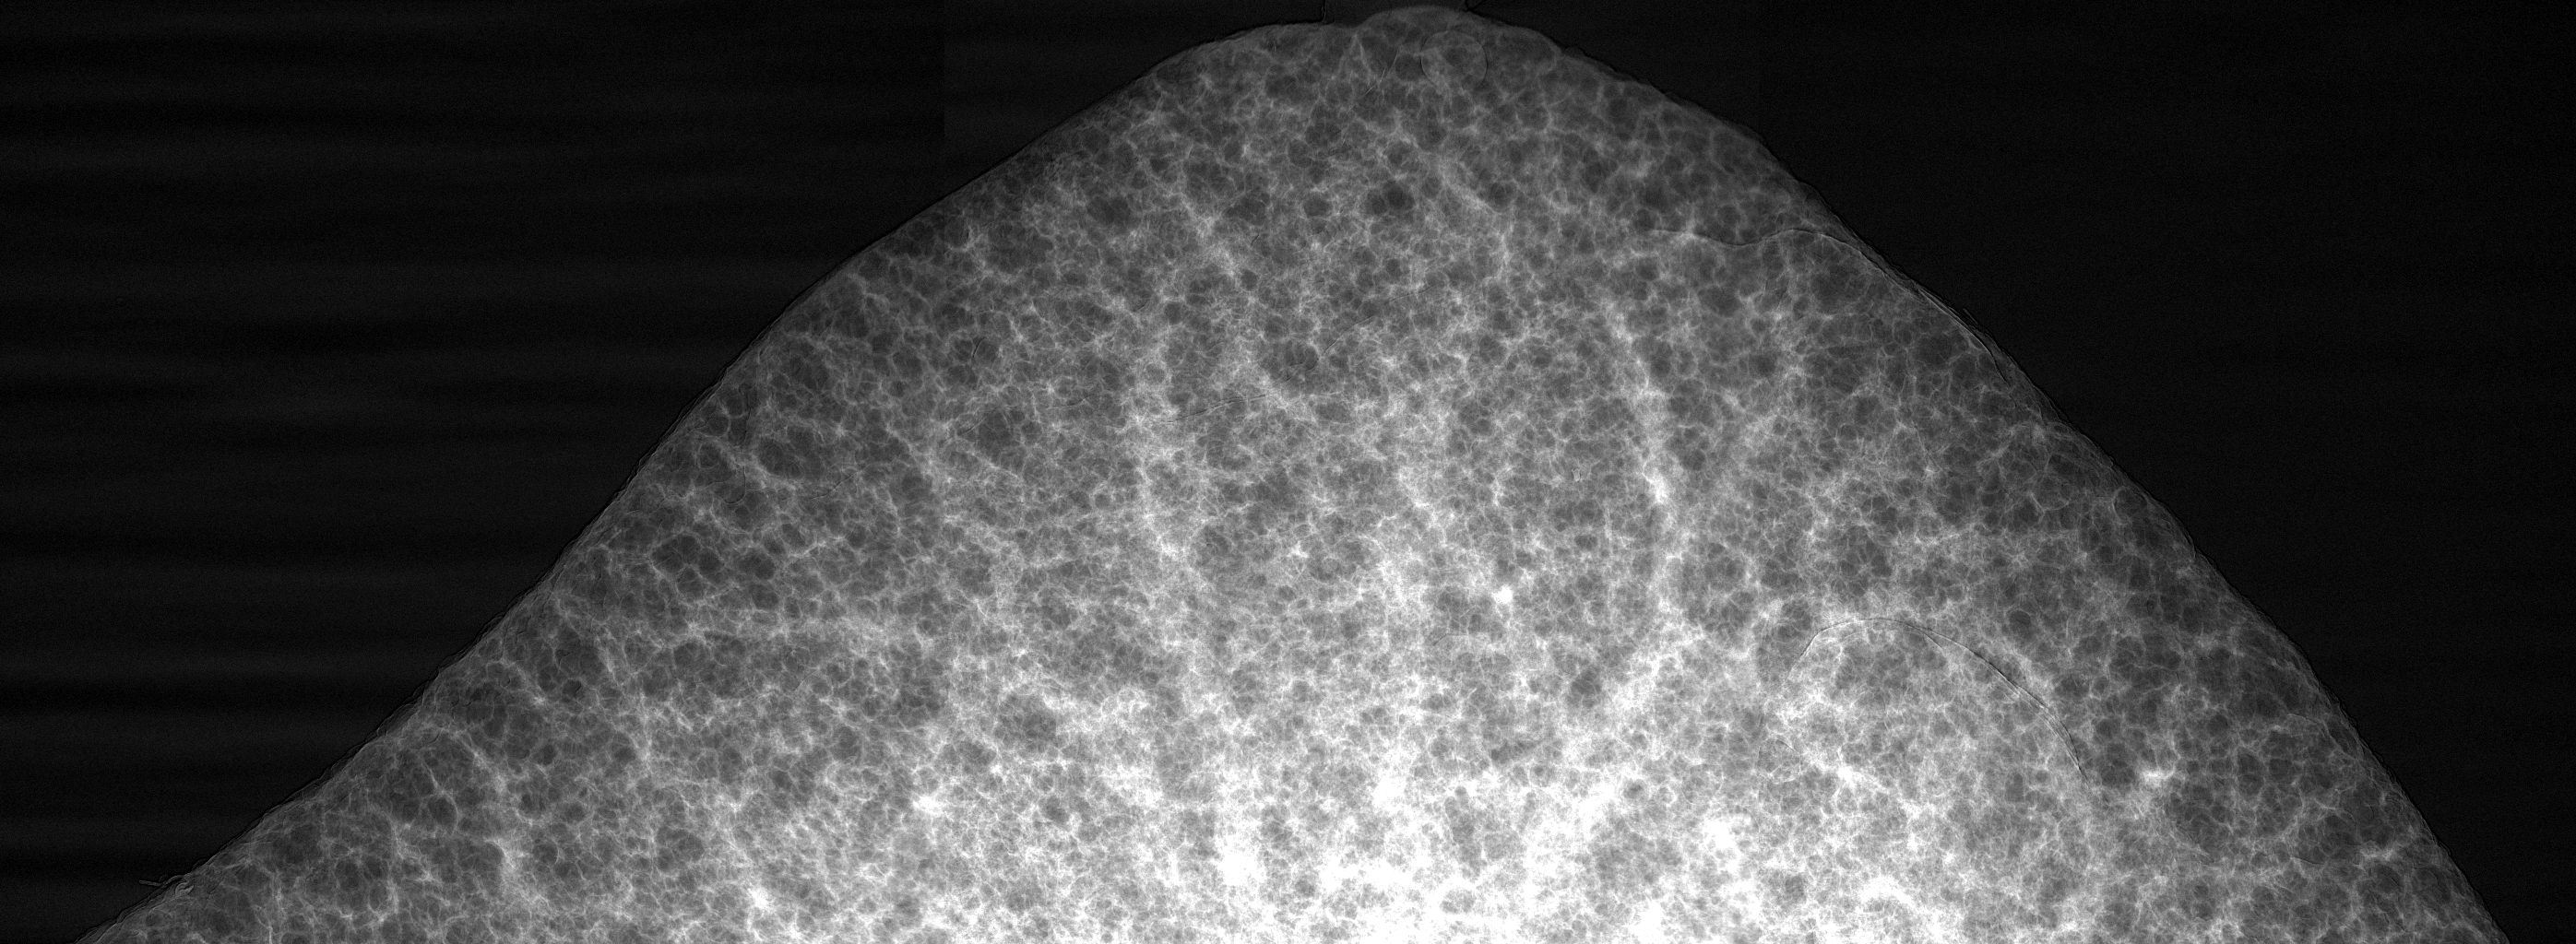
\includegraphics[width=\imagewidth]{R108C21Cb_mrg3333_normalize}};%
				\def\x{2693} % 2793-100
				\def\y{922} % 1024*.9 = 921.6
				\def\bar{338} % 100 px = 148 um
				\draw[|-|,color=white] (1,256) -- (2792,256) node [midway,above] {\SI{4.13364}{\milli\meter}};
				\draw[|-|,color=white] (\x-\bar,\y) -- (\x,\y) node [midway,above] {\SI{500}{\micro\meter}};
				\end{tikzpicture}%
			\label{fig:merge-proj}%
			}\\%
		\renewcommand{\imsize}{\linewidth}%
		\pgfmathsetlength{\imagewidth}{\imsize}% desired displayed width of image
		\pgfmathsetlength{\imagescale}{\imagewidth/2792}% pixel width of image (image has been resized from 2994*1123, so that scalebar is at the same height without calculating too much...)
		\subfloat[Cropped part of one slice of the tomographic dataset reconstructed from 5244 merged projections shown in subfigure~\subref{fig:merge-proj}. Due to the coherence of the x-ray beam the air-to-paraffin interface is visible around the sample.]{%
			\begin{tikzpicture}[x=\imagescale,y=-\imagescale]%
				% place image (integer coordinates refer to pixel centers):
				\node [anchor=north west,inner sep=0pt,outer sep=0pt] at (0,0)%
					{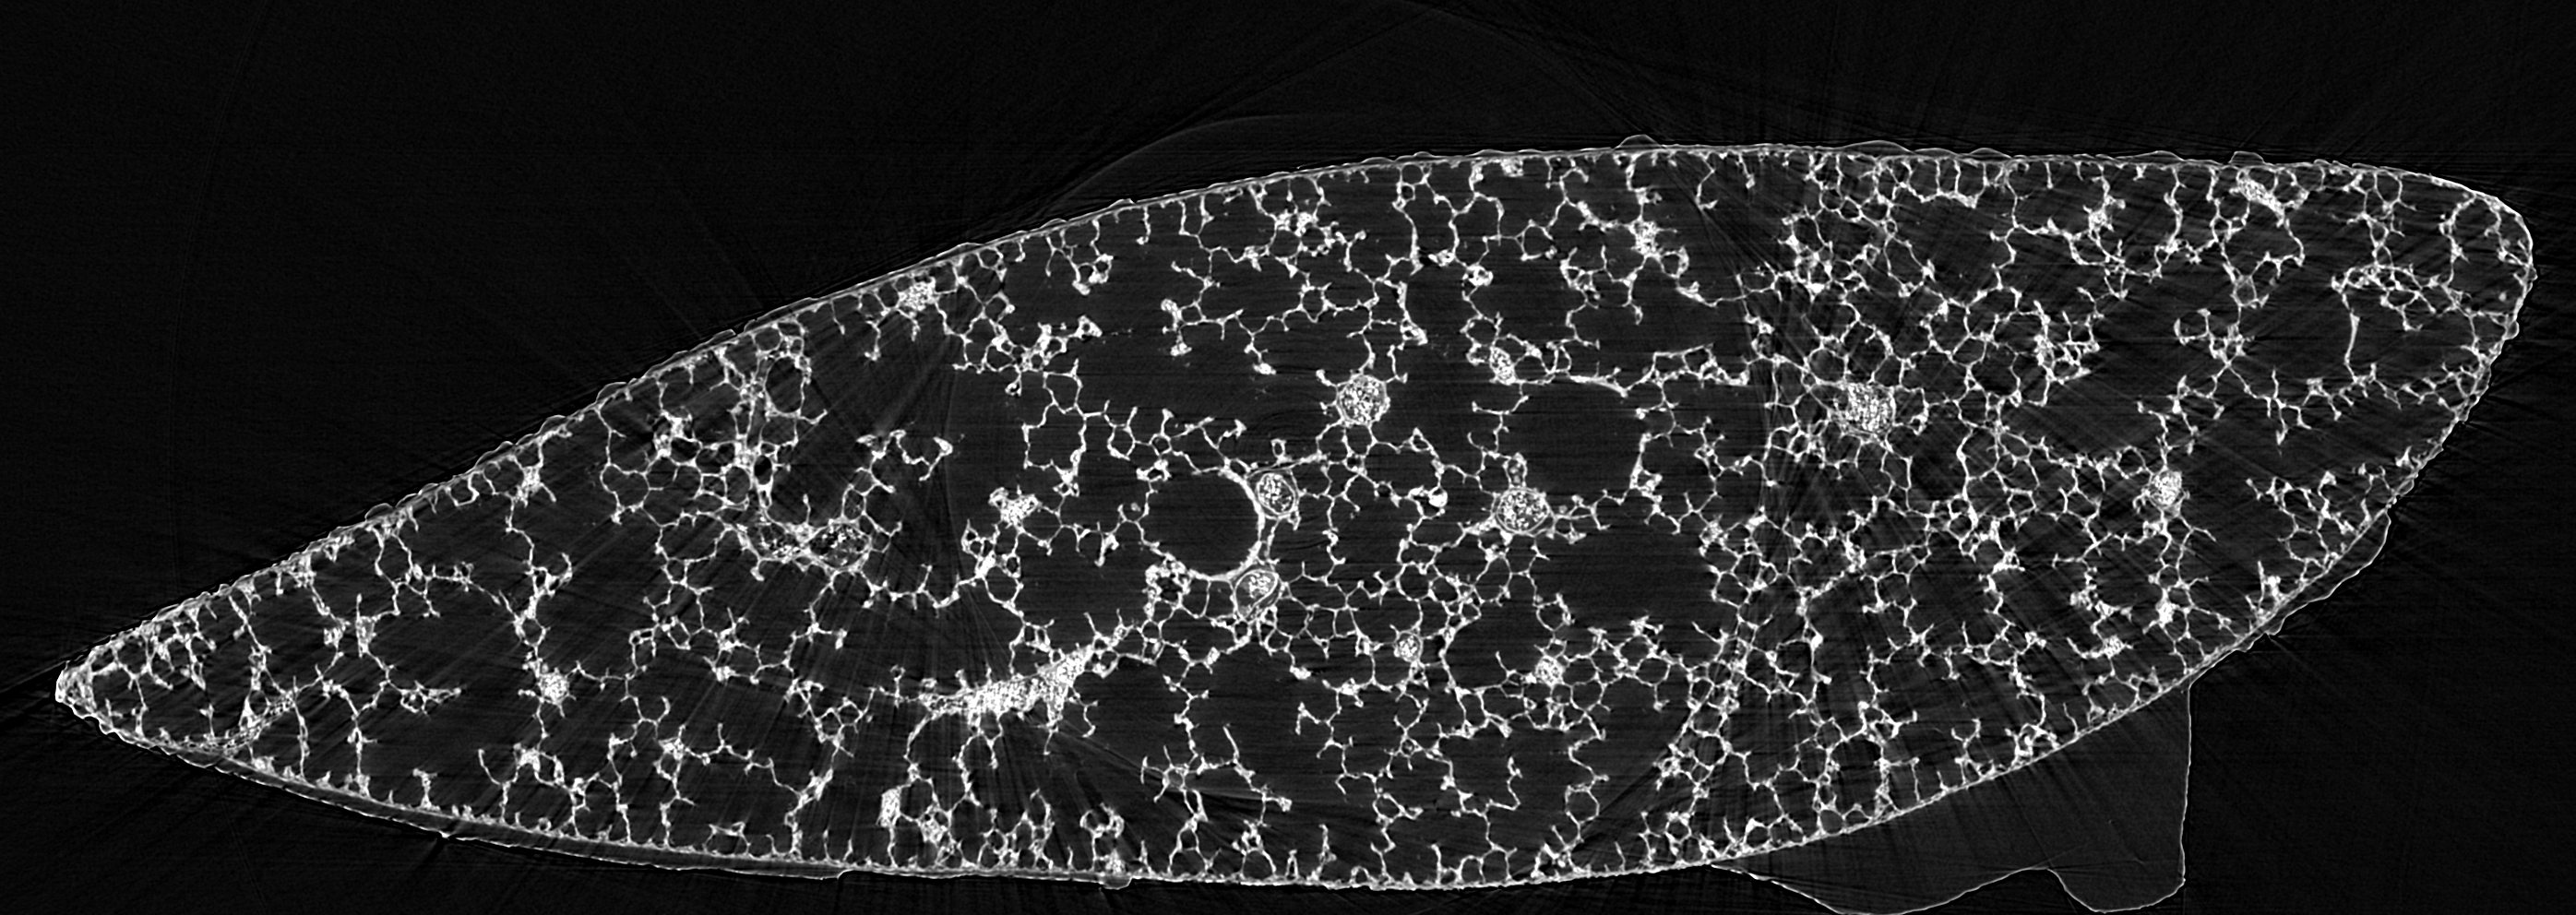
\includegraphics[width=\imagewidth]{R108C21Cb_mrg1024rec8bit}};% ``mogrify -shave 0x900 -normalize -format png R108C21Cb_mrg1024rec8bit.tif''
				\clip (0,0) rectangle (2792,992);				
				\def\x{2692} % 2708-100
				\def\y{893} % 992 * .9 = 892.8
				\def\bar{338} % 100 px = 148 um
				%%%% scalebar
					\draw[|-|,color=white] (\x-\bar,\y) -- (\x,\y) node [midway,above] {\SI{500}{\micro\meter}};
					\draw[|-|,color=white] (1,20) -- (2792,20) node [midway,below] {\SI{4.13216}{\milli\meter}};
				%%%% center
					\fill [color=red] (2792/2,992/2) circle (5);
				%%%% big circle
					\draw [dashed,color=red] (2792/2,992/2) circle (512);
					\def\angle{45}
					\draw [white,<->] (2792/2,992/2) +(\angle:0) --  node (bigto) {} +(\angle:512); 
					\node [white] (bigfrom) at (256,256){$\frac{1024}{2}$px};
					\draw [white,->,densely dotted] (bigfrom) to [bend left=45] (bigto);
				%%%% big circle
				%%%% 141px circle
				\draw [dashed,color=red] (2792/2,992/2) circle (512-141);
				\def\angle{45+90}
					\draw [white,<->] (2792/2,992/2) +(\angle:0) -- node (smallto) {} +(\angle:512-141);
					\node [white] (smallfrom) at (256,384) {$\frac{1024}{2}-141$px};
					\draw [white,->,densely dotted] (smallfrom) to [bend left=45] (smallto);
				%%%% 141px circle					
%				%%%% 138px circle
%				\draw [dashed,color=red] (2792/2,992/2) circle (512-138);
%				\def\angle{45+90+90}
%					\draw [white,<->] (2792/2,992/2) +(\angle:0) -- node (vsmallto) {} +(\angle:512-138);
%					\node [white] (vsmallfrom) at (2972-768,992-512) {$\frac{1024}{2}-138$px};
%					\draw [white,->,densely dotted] (vsmallfrom) to [bend right=45] (vsmallto);
%				%%%% 138px circle
				%%%% inset
%				\newcommand{\size}{.2\imagewidth}%
%				\clip (256,256) rectangle (512,512);
%				\node[anchor=north west,inner sep=0pt,outer sep=0pt] at (0,0)
%					{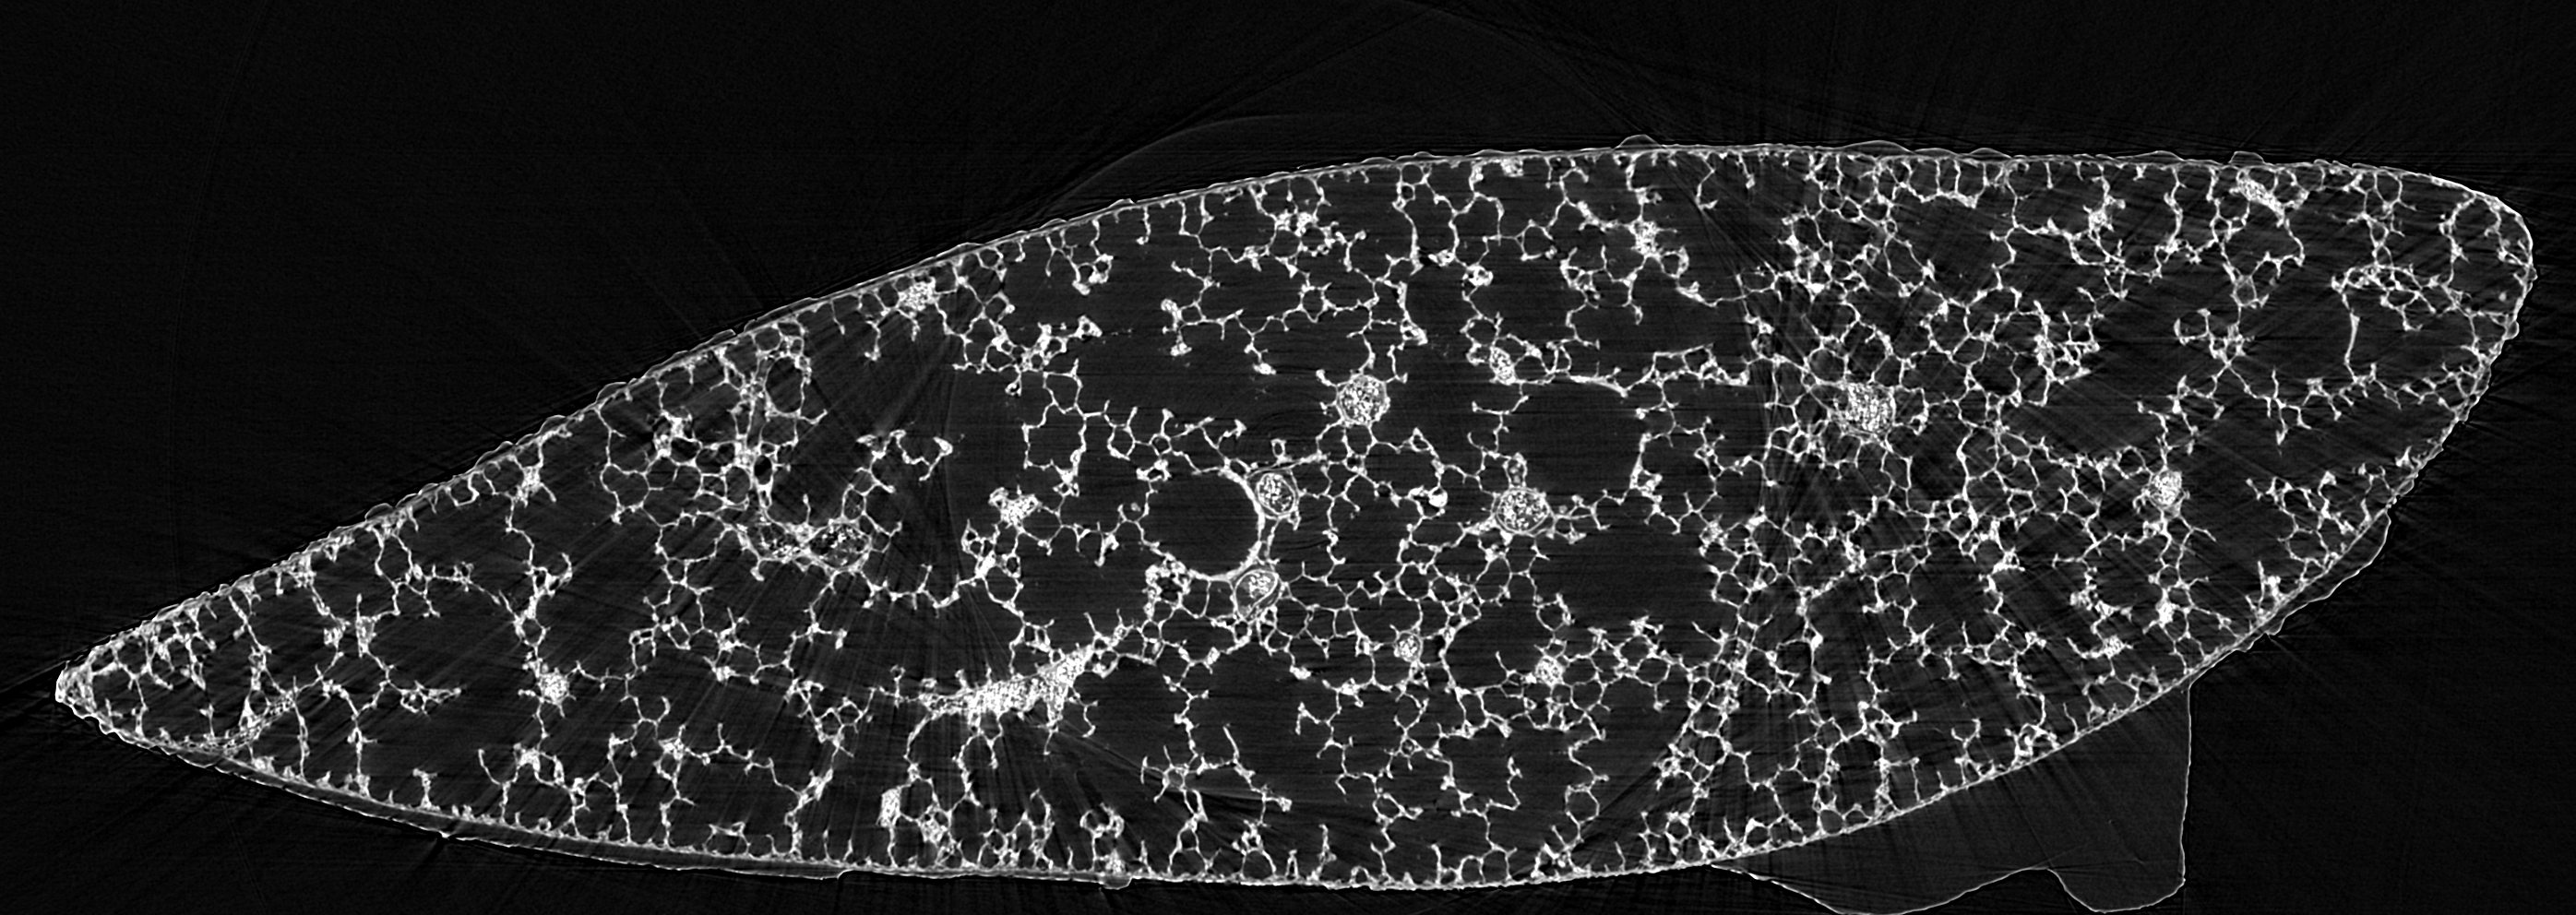
\includegraphics[width=\size]{R108C21Cb_mrg1024rec8bit}};
%					\draw[white] (0,0) rectangle (\size,-\size);
				%%%% inset
				\end{tikzpicture}%
			\label{fig:merge-rec}%
			}%
%%%%%%%%%%%%%%%%%%%%%%%%%%%%%	
%	\caption{caption}
%\end{figure}
%\end{document}